
\section*{CHƯƠNG 2. PHÂN TÍCH HỆ THỐNG}
\setcounter{section}{2}
\setcounter{subsection}{0} %LƯU Ý MỖI LẦN THÊM CHƯƠNG MỚI CẦN THÊM CÂU NÀY ĐỂ RESET THỨ TỰ CỦA SUBSECTON VỀ 1
\setcounter{table}{0} % LƯU Ý SAU MỖI LẦN GỌI BẢNG HAY HÌNH ẢNH PHẢI THÊM CÂU NÀY ĐỂ RESET THỨ TỰ
\setcounter{figure}{0} %% LƯU Ý SAU MỖI LẦN GỌI BẢNG HAY HÌNH ẢNH PHẢI THÊM CÂU NÀY ĐỂ RESET THỨ TỰ
\addcontentsline{toc}{section}{\numberline{}CHƯƠNG 2. PHÂN TÍCH HỆ THỐNG}
Trong chương này, chúng em sẽ tiến hành phân tích hệ thống cho dự án đề tài "Hệ thống theo dõi và quản lý dữ liệu điện tim" dựa trên các mục tiêu
đã nêu ra trong Mục Đề xuất hệ thống ở Phần mở đầu. Trước tiên bài toán đặt ra ở hệ thống là:
\begin{adjustwidth}{1.5em}{}
\begin{itemize}
  \item Một ứng dụng để có thể giúp người dùng/bệnh nhân theo dõi được những thông tin cần về sức khoẻ tim mạch
  \item Trực quan và tiêu chuẩn hoá những thông tin đo được
    bằng hình ảnh hoặc số liệu để bác sĩ có thể dựa vào đó để đưa ra những đánh giá cho người dùng. Ngoài ra những thông tin này
    có thể hữu ích trong việc theo dõi sức khỏe tim mạch, theo dõi hiệu quả của liệu pháp 
    và hỗ trợ quyết định của người dùng
  \item Quản trị viên sẽ là người có thể phân công bác sĩ để chăm sóc, theo dõi sức khoẻ từ
  xa cho bệnh nhân
\end{itemize}
\end{adjustwidth}
Chi tiết về việc phân tích các yêu cầu hệ thống sẽ được chúng em trình bày ở các chương dưới.

\subsection{Sơ đồ use case}
\subsubsection{Use case tổng quát hệ thống}
Dựa vào những phân tích về yêu cầu chức năng, các use case trong hệ thống được chúng em thể hiện ở hình dưới 
  \begin{figure}[H]
    \centering
    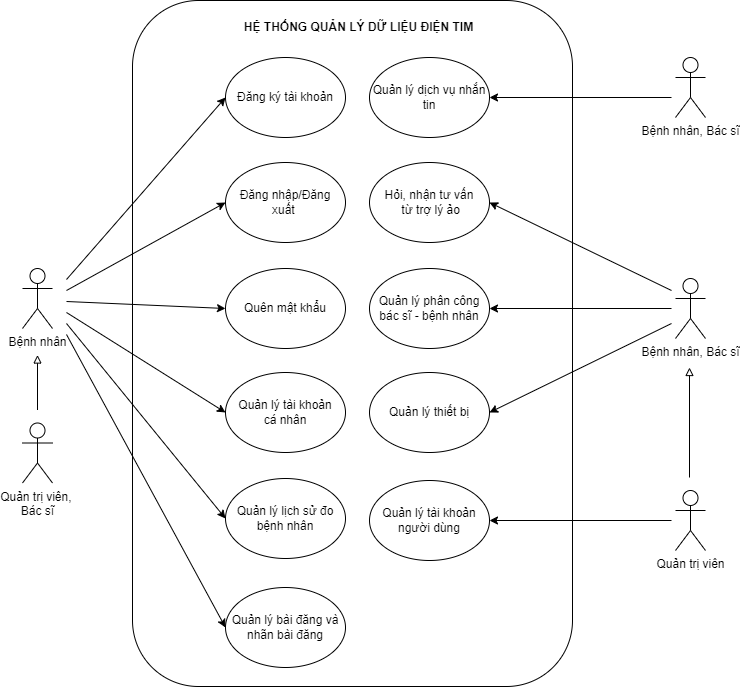
\includegraphics[width=16cm,height=14cm]{Images/use_case/use_case_general.png}
    \caption[Sơ đồ use case tổng quát của hệ thống]{\bfseries \fontsize{12pt}{0pt}
    \selectfont Sơ đồ use case tổng quát của hệ thống}
    \label{use_case_general} %đặt tên cho ảnh
  \end{figure}

\subsubsection{Use case chức năng xem lịch sử các lần đo}
  \begin{figure}[H]
    \centering
    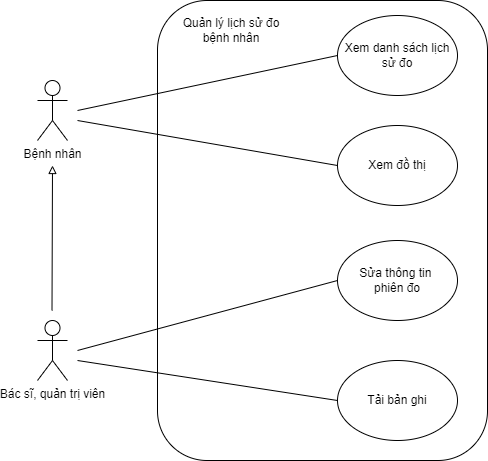
\includegraphics[width=12cm,height=4.8cm]{Images/use_case/use_case_view_history_record.png}
    \caption[Sơ đồ use case chức năng xem lịch sử các lần đo]{\bfseries \fontsize{12pt}{0pt}
    \selectfont Sơ đồ use case chức năng xem lịch sử các lần đo}
    \label{use_case_view_history_record} %đặt tên cho ảnh
  \end{figure}

  \begin{table}[H]
    \caption{\bfseries \fontsize{12pt}{0pt}\selectfont Bảng phân tích use case chức năng xem lịch sử các lần đo}
    \centering
    \begin{tabularx}{0.9\textwidth}{|c|X|}
      \hline
      \textbf{Tên chức năng} & \textbf{Xem lịch sử các lần đo} \\
      \hline
      Tác nhân & Bệnh nhân, Bác sĩ \\
      \hline
      Mô tả & Cho phép bệnh nhân xem lịch sử các lần đo điện tim và bác sĩ xem được lịch sử các lần đo của bệnh nhân
      mà mình quản lý \\
      \hline
      Điều kiện trước & Người dùng cần có kết nối Internet và đã đăng nhập \\
      \hline
      Dòng sự kiện chính & 
      % \begin{tabular}{@{}l@{}}
        Chi tiết luồng sự kiện được thể hiện ở Hình \ref{view_record_timeline}, Hình \ref{getEcgRecordsByUserId}, Hình \ref{getEcgRecordsByDoctor} 
        \\
      % \end{tabular} \\
      \hline
    \end{tabularx}
  \end{table}
% \newpage
\subsection{Thẻ CRC (Class - Responsibility - Collaboration Card)}

% \newpage
\subsection{Sơ đồ lớp}

% \newpage
\subsection{Sơ đồ tuần tự}
Để phân tích cụ thể hơn từng luồng trong hệ thống qua use case, chúng em xin phép được trình bày các sơ đồ tuần
tự. 
\subsubsection{Sơ đồ tuần tự chức năng đăng ký}
  \begin{figure}[H]
        \centering
        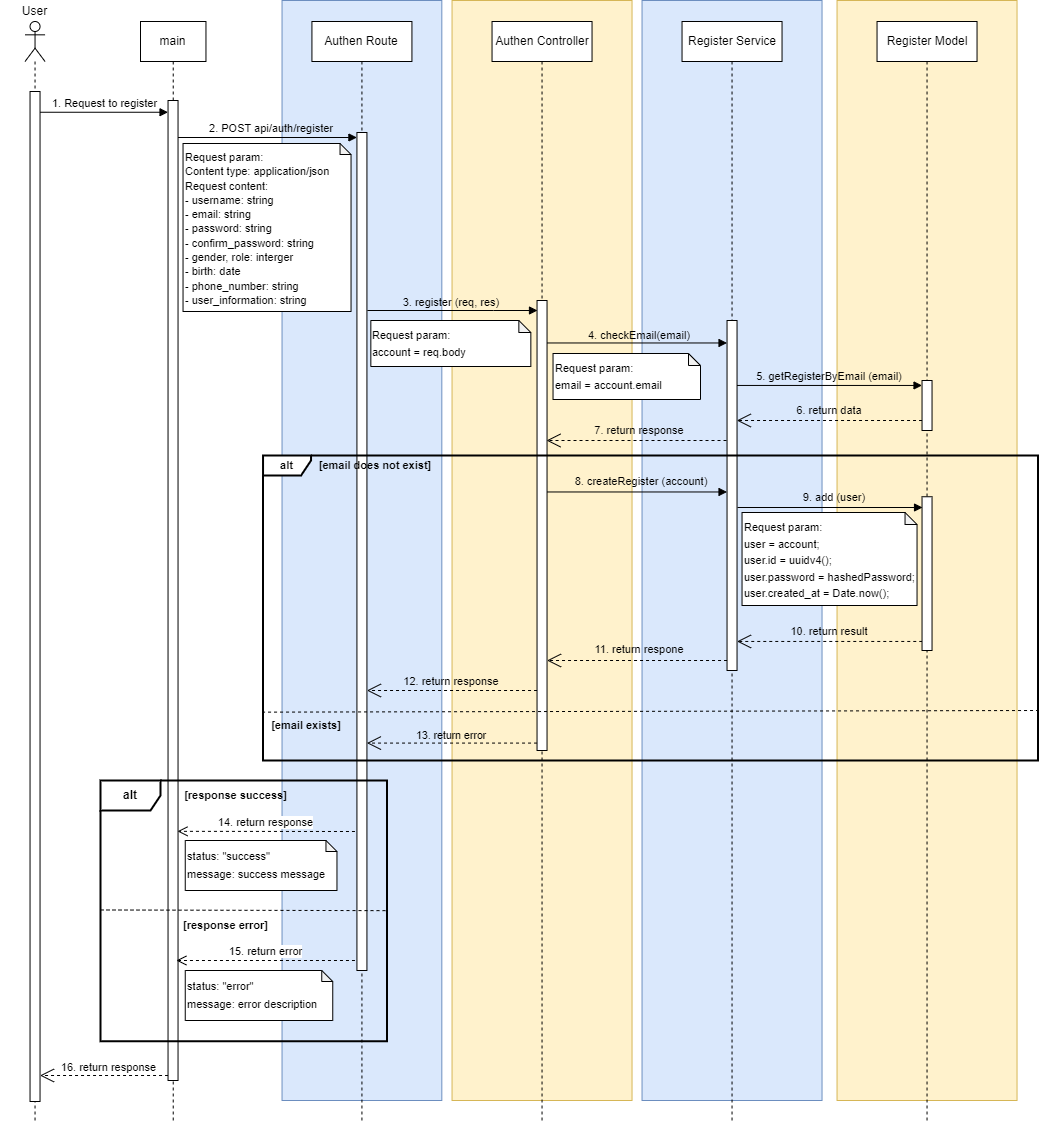
\includegraphics[width=12.9cm,height=9.4cm]{Images/mobile_app/register.png}
        \caption[Sơ đồ tuần tự chức năng đăng ký trên App]{\bfseries \fontsize{12pt}{0pt}
        \selectfont Sơ đồ tuần tự chức năng đăng ký trên App}
        \label{register} %đặt tên cho ảnh
  \end{figure}
  Sơ đồ tuần tự trên mô tả chi tiết quá trình người dùng đăng ký vào hệ thống. Người dùng gửi yêu cầu đăng ký, yêu cầu sẽ
  được xử lý bởi Control, nếu có lỗi phát sinh sẽ trả ra lỗi cho người dùng và yêu cầu người dùng nhập lại. Control
  sẽ xử lý cụ thể như thế nào được chúng em thể hiện trong Hình \ref{backend_register} trong chương sau.
\subsubsection{Sơ đồ tuần tự chức năng đăng nhập/đăng xuất}

    \begin{figure}[H]
         \centering
         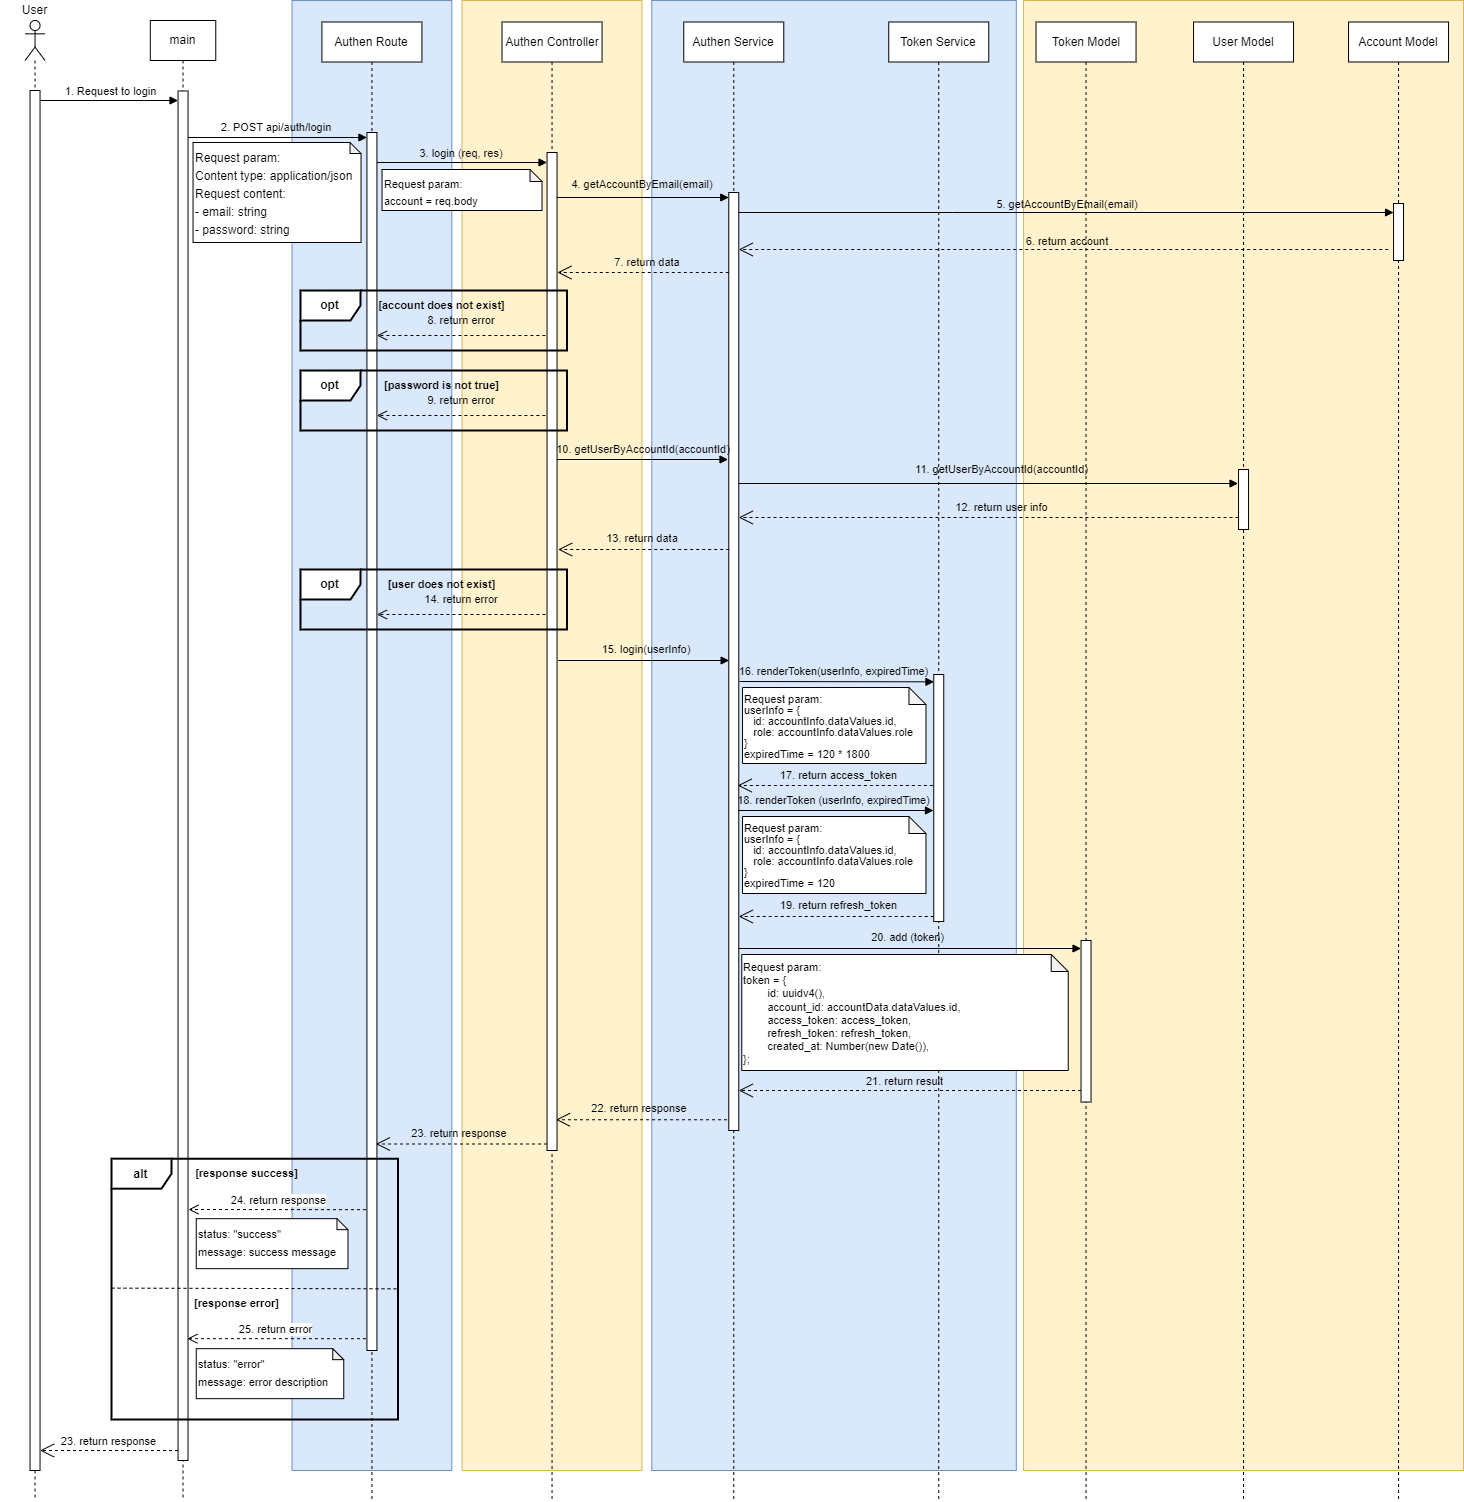
\includegraphics[width=16cm,height=12cm]{Images/mobile_app/login.png}
         \caption[Sơ đồ tuần tự chức năng đăng nhập trên App]{\bfseries \fontsize{12pt}{0pt}
         \selectfont Sơ đồ tuần tự chức năng đăng nhập trên App}
         \label{login} %đặt tên cho ảnh
    \end{figure}

  Sơ đồ tuần tự trên mô tả chi tiết quá trình người dùng đăng nhập vào hệ thống. Người dùng gửi yêu cầu đăng nhập, yêu cầu sẽ
  được xử lý bởi Control, nếu có lỗi phát sinh sẽ trả ra lỗi cho người dùng và yêu cầu người dùng nhập lại. Việc Control
  sẽ xử lý cụ thể yêu cầu người dùng được chúng em thể hiện trong Hình \ref{backend_login} trong chương sau.

  \begin{figure}[H]
    \centering
    \includegraphics[width=12cm,height=6cm]{Images/mobile_app/logout.png}
    \caption[Sơ đồ tuần tự chức năng đăng xuất trên App]{\bfseries \fontsize{12pt}{0pt}
    \selectfont Sơ đồ tuần tự chức năng đăng xuất trên App}
    \label{logout} %đặt tên cho ảnh
\end{figure}

Sơ đồ tuần tự trên mô tả chi tiết quá trình người dùng đăng xuất khỏi hệ thống. Người dùng gửi yêu cầu đăng xuất, yêu cầu sẽ
được xử lý bởi Control, nếu có lỗi phát sinh sẽ trả ra lỗi cho người dùng và yêu cầu người dùng nhập lại. Việc Control
sẽ xử lý cụ thể yêu cầu người dùng được chúng em thể hiện trong Hình \ref{backend_logout} trong chương sau.

\subsection{Phân tích dữ liệu}

Tại phần này, chúng em sẽ tiến hành xác định và mô tả các thực thể cũng như
 thuộc tính quan trọng trong hệ thống. Việc này giúp chúng ta có cái
  nhìn tổng quan về các yếu tố chính cần được quản lý và lưu trữ
   trong cơ sở dữ liệu. Bằng cách làm điều này, chúng ta có thể
    xây dựng một mô hình dữ liệu cơ bản để hỗ trợ việc thiết kế và
     triển khai hệ thống một cách hiệu quả.

     Trước hết, chúng em sẽ xác định và mô tả các thực thể chính trong hệ
      thống. Thực thể là các đối tượng hoặc khái niệm quan
       trọng mà chúng ta cần theo dõi và quản lý. Sau đó, chúng ta sẽ xác
        định các thuộc tính liên quan đến mỗi thực thể, các thông tin cần
         được lưu trữ và quản lý.

\begin{table}[H]
  \caption{\bfseries \fontsize{12pt}{0pt}\selectfont Bảng thực thể và thuộc tính}
  \centering
  \begin{tabularx}{0.9\textwidth}{|c|X|}
    \hline
    \textbf{Thực thể} & \textbf{Thuộc tính} \\
    \hline
    Người dùng & 
    ID người dùng, Mật khẩu, Email, Tên, Ngày sinh, Số điện thoại, Quyền \\
    \hline
    Bản ghi ECG & 
    ID bản ghi ECG, ID người dùng, ID thiết bị, Đường dẫn lưu trữ dữ liệu, Thời gian bắt đầu đo, Thời gian kết thúc đo, Loại cảm biến \\
    \hline
    Danh mục tin tức & 
    ID danh mục tin tức, Tên danh mục tin tức, Mô tả danh mục tin tức \\
    \hline
    Tin tức & 
    ID tin tức, Tiêu đề, Nội dung, ID danh mục tin tức, Tác giả, Đường dẫn, Đường dẫn hình ảnh \\
    \hline
    Phân công bệnh nhân - bác sĩ & 
    ID phân công, ID bệnh nhân, ID bác sĩ, Ngày bắt đầu \\
    \hline
    Mã thông báo đặt lại mật khẩu & 
    ID mã thông báo, ID người dùng, Mã thông báo, Thời gian hết hạn \\
    \hline
    Phiên đăng nhập & 
    ID phiên đăng nhập, ID người dùng, Mã phiên đăng nhập, Thời gian hết hạn \\
    \hline
    Thiết bị & 
    ID thiết bị, Tên thiết bị \\
    \hline
    Thông tin hội thoại & 
    ID hội thoại, Danh sách ID người dùng trong hội thoại, thông tin tin nhắn gần nhất \\
    \hline
    Tin nhắn & 
    ID tin nhắn, Nội dung tin nhắn, ID người gửi tin nhắn, thời gian gửi tin nhắn \\
    \hline
    Firebase token người dùng & 
    ID token, Firebase token, ID người dùng \\
    \hline
  \end{tabularx}

  
\end{table}
Sau khi hoàn thành được bảng thực thể và thuộc tính, chúng em xác định được mô hình thực thể liên kết như sau:

\begin{figure}[H]
  \centering
  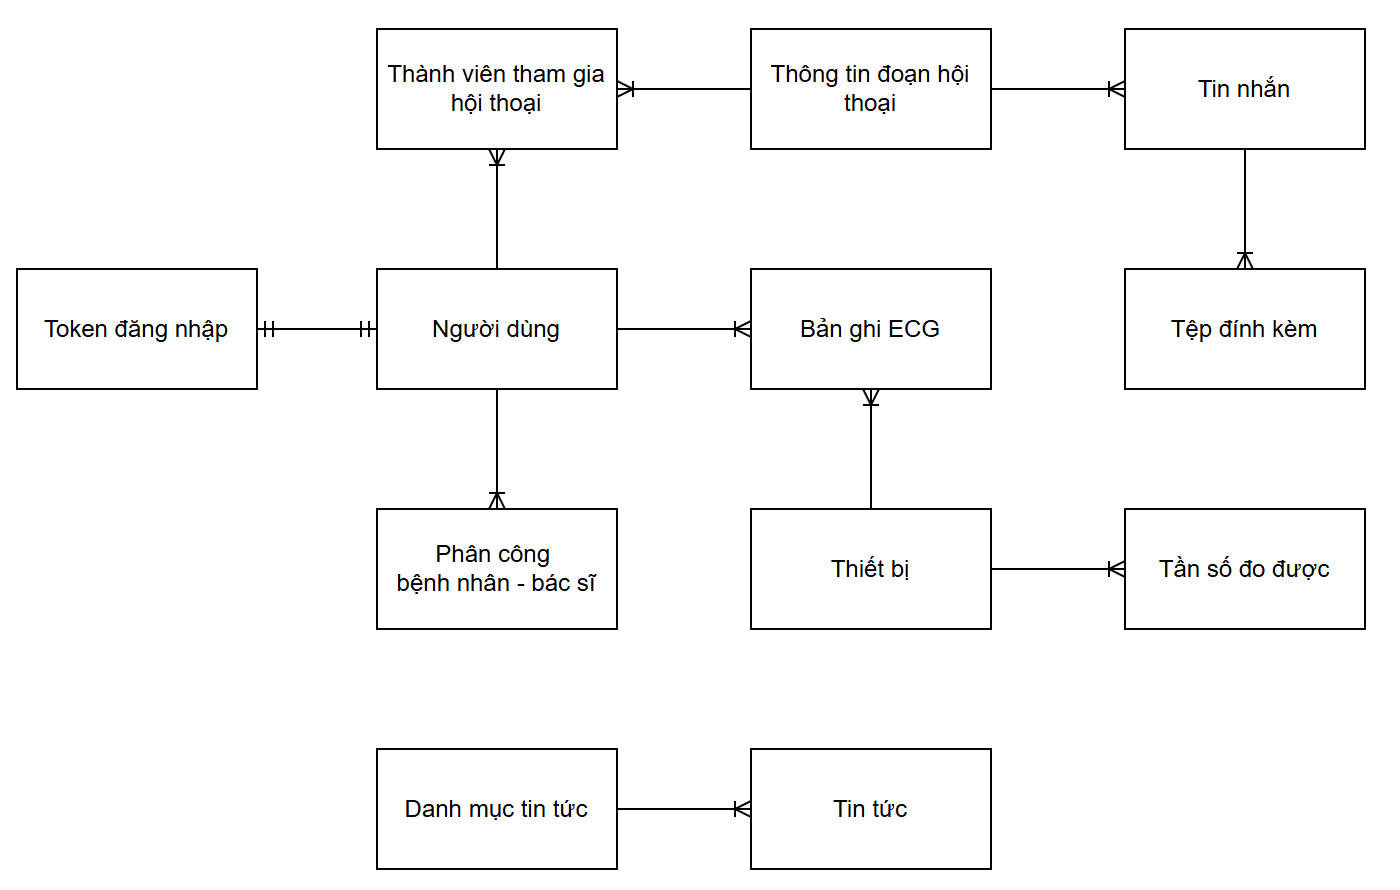
\includegraphics[width=15cm,height=8cm]{Images/system/fmECG_connection_entity.png}
  \caption[Mô hình thực thể liên kết]{\bfseries \fontsize{12pt}{0pt}
  \selectfont Mô hình thực thể liên kết}
  \label{ttlk} %đặt tên cho ảnh
\end{figure}


\subsection{Kết luận chương}

Trong chương này, chúng em đã thực hiện phân tích toàn diện về
 hệ thống cho đề tài , nhằm đáp ứng
  các mục tiêu và yêu cầu đã được đề xuất.

Chúng em đã xác định rõ ràng các khía cạnh quan trọng của hệ thống,
 tập trung vào việc thiết kế một hệ thống quản lý ECG hiệu quả,
  trực quan và có khả năng theo dõi sức khỏe tim mạch một cách
   chính xác. 


\newpage
